\newsection

\subsection{BP 9:
 Okushiri Island (Field)} \label{sec:bp9}

{\bf Documentation:}
\begin{itemize} 
\item PMEL-135, pp 8 \& 48-53 \cite{SynolakisBernard:pmel135}.
\item A problem description is provided by Frank Gonz\'alez 
 at \cite{bp-description}:\\
\href{https://github.com/rjleveque/nthmp-benchmark-problems/blob/master/BP09-FrankG-Okushiri\_island/Description.pdf} 
{BP09-FrankG-Okushiri\_island/Description.pdf} 
\item Numerous other publications also describe this event, in varying detail: 
\cite{DCRC1994,HTSG1993,KatoTsuji1994,TakahashiEtAl1995,Takahashi1996}
\end{itemize} 

\subsubsection{Description}
The goal of this Benchmark Problem (BP) is to compare computed model results with field observations of the 1993 Okushiri Island tsunami.

\subsubsection {Problems encountered}
Two basic problems were encountered:
\begin {enumerate}
\item Poor quality of the computational bathymetric/topographic grids
\item Inaccurate spatial registration of field observational data with the model grids. 
\end{enumerate} 

\subsubsection{What we did}

\begin{itemize}
\item Used g = 9.81 and Manning coefficient 0.025 for the friction term.  We
also ran many of the tests with no friction for comparison.  
\item Used bathy/topo grids and source grid for the Disaster Control Research Center solution DCRC17a.  Dmitry Nicolsky provided improved versions of the originals developed by Kansai University, in which severe misalignments in the original data were reduced (but not eliminated).
\end{itemize}

\subsubsection{Problem Requirements}
  Requirements of this benchmark test were to compute:
\begin{enumerate}
\item  Runup around Aonae
\item  Arrival of the first wave to Aonae
\item  Two waves at Aonae approximately 10 min apart; the first wave from the west, the second from the east
\item  Water level at Iwanai and Esashi tide gauges
\item  Maximum modeled runup distribution around Okushiri Island
\item  Modeled runup height at Hamatsumae
\item  Modeled runup height at a valley north of Monai
\end{enumerate}

\subsubsection{Results}

Figures \ref{bp9full} through  \ref{bp9inaonae} show results of one computation where AMR is used to concentrate grid points near the southern Aonae Peninsula and  (Requirements 1, 2, 3). The rectangular boxes show regions of refinement.  The coarsest grid is a $60\times 60$ grid on a 1-degree square as shown in Figure \ref{bp9full}. Five levels of refinement are used going down by factors 2, 4, 4, and 6 from each level to the next. In this computation, Level 4 is only allowed on the southern half of Okushiri Island and Level 5 only around the Aonae Peninsula. 

Figure \ref{bp9ok} shows a zoom on the island and Figure \ref{bp9aonae} a further zoom on the peninsula.  Arrival of the first wave at Aonae (Requirement 2) is seen from the west at about $t = 5$ minutes.  The second major wave arrives from the east at about 10 minutes.    

Figure \ref{bp9inaonae} shows the inundation level on the peninsula.  The color scale indicates the maximum depth of water recorded at each point on a fixed grid that is placed around this region.  This can be compared to the photographs shown in Figure \ref{bp9photos}.

A slight modification of this run was done to focus on the Hamatsumae  region just east of the peninsula.  Figure \ref{bp9hama} shows the maximum inundation in this region.

 % the subsequrent runup around Aonae (Requirement 1) is presented in Figure \ref{AonaeRunup}.  The first wave arrived at about t = 5 minutes, and wrapped around the peninsula, engulfing Aonae proper in about 2 minutes, at t = 7 minutes, as seen in Figure \ref{Aonae07min.png}.  Between 9 and 10 minutes later, at t=16 and 17 minutes, Hamatsumae (\ref{Aonae16min.png} and then the northeastern coast of the Aonae peninsula \ref{Aonae17min.png} are inundated by a wave from the east (Requirements 3 and 6).  Figures \ref{WestObsVsGeoClaw} and \ref{EastObsVsGeoClaw} present the observed and modeled maximum runup distribution on the West and East coasts of Okushiri, respectively (Requirement 5), including a valley north of Monai where the observed runup height that exceeded 30 m \ref{WestObsVsGeoClaw} (Requirement 7).  Figures \ref{Iwanai} and \ref{Esashi} present the model results and tide gage time series at Iwanai and Esashi.  The correspondence of model and observed tides is poor at both locations, perhaps due to the issue of inaccurate spatial registration of the tide gage positions and the corresponding computational grid cell.  

The bottom panel of Figure \ref{TeamStations} shows the runup at various other points around the island as measured by the team of Y. Tsuji (top panel), along with values computed using GeoClaw.  Figure \ref{bp9scatter} shows a scatter plot of the correlation between the observations and the computed values.  The GeoClaw values were obtained by placing a small fixed grid around each observation point and recording the maximum water depth at each point on this grid at each timestep of the computation, using the built-in feature of GeoClaw.  The maximum depth over time can also be accumulated at these points and updated each time step.  Plots of the maxima over these grids gives a visualization of the maximum extent of inundation.  Such plots are shown  in Figures \ref{bp9inaonae} and \ref{bp9monai}, with 4-meter contours.  For most other observation  points contours of topography at 2-meter increments were plotted in order to better estimate the maximum runup in a small region centered about each observation point. 
%Figure \ref{bp9fg} shows a sample of several of these inundation maps. 

Figure \ref{bp9monai} shows the inundation map for the Valley north of Monai, with 4-meter contour lines (Requirement 7).  Inundation to roughly 32 m is observed, in accordance with observations.  For this run a finer grid was used in the region around the value (refining by a factor 24 rather than 6 in the level 5 grid), and the finer scale bathymetry provided in this region was used.

Requirement 4 is the comparison of observed and computed water level at the Iwanai and Esashi tide gage stations; the analog records are shown in Figure \ref{TGs-Takahashi}, taken from \cite{TakahashiEtAl1995}.  The digitized tide gage data are compared with the GeoClaw time series in Figures \ref{Iwanai} and \ref{Esashi}.  At Iwanai, the digitized tide gage record is clearly undersampled (compare Figures \ref{TGs-Takahashi} and \ref{Iwanai}), but does capture the peaks and troughs of the analog record.  We see that the first wave arrival time and the overall wave amplitudes are comparable, but that the GeoClaw tsunami waves are about half the period of the waves recorded by the Iwanai tide gage.  Considering the regularity of the long train of waves in the tide gage record, it is probable that longer period resonance modes at Iwanai were excited by the incident tsunami; if so, then higher resolution bathy/topo grids would be required to capture these resonant oscillations in a numerical simulation.  At Esashi, it appears that the digitized tide record reflects the main features of the analog record (compare Figures \ref{TGs-Takahashi} and \ref{Esashi}).  However, the strange shape of the analog wave form makes it likely that there are problems with the tide gage record; the record suffers from either mechanical/electronic, or damage by debris, or simply a damped and/or mismatched response function in the tsunami frequency band.  In spite of this, the first arrival and timing of the first two tsunami waves are in good correspondence, though the amplitude and individual wave forms are not.

%-------------

\begin{figure}[ht]
\hfil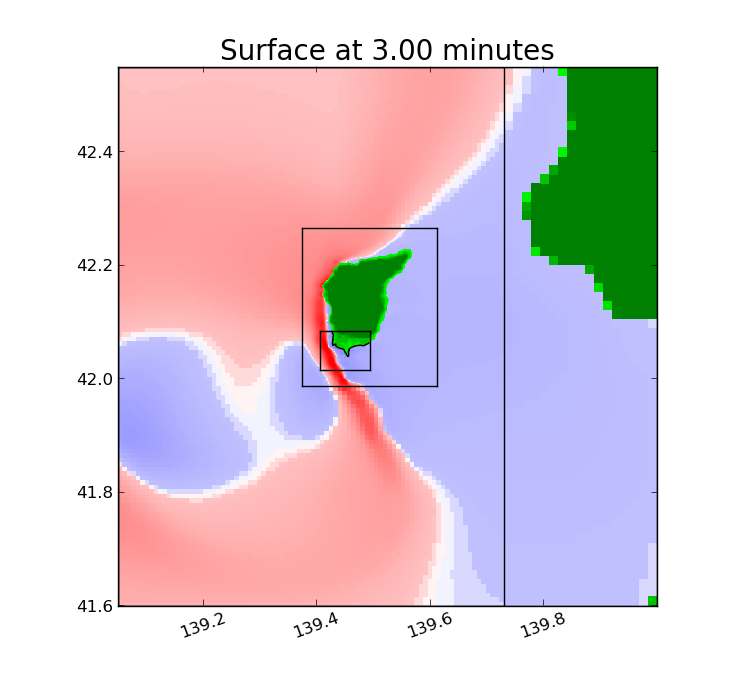
\includegraphics[width=2.8in]{bp9/full_3min.png}\hfil
\hfil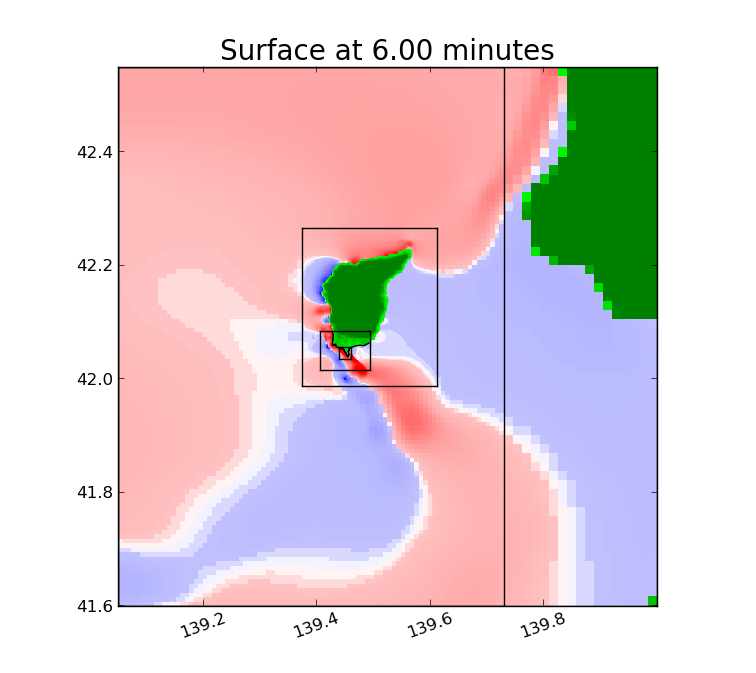
\includegraphics[width=2.8in]{bp9/full_6min.png}\hfil

\caption{\label{bp9full}
Full computational domain for one simulation, in which AMR grids are focused near the Aonae Peninsula at the south of Okushiri Island.
  }
\end{figure}

\begin{figure}[ht]
\hfil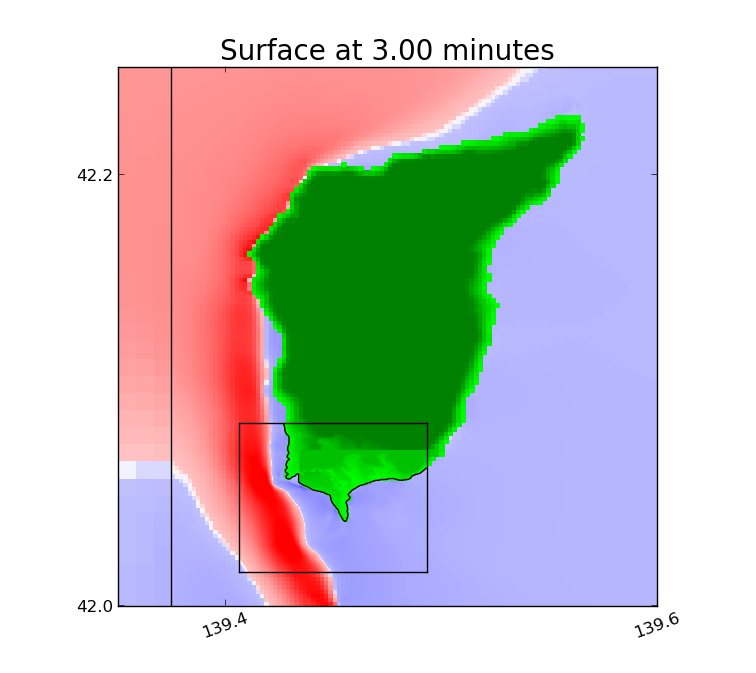
\includegraphics[width=2.0in]{bp9/ok_3min.png}\hfil
\hfil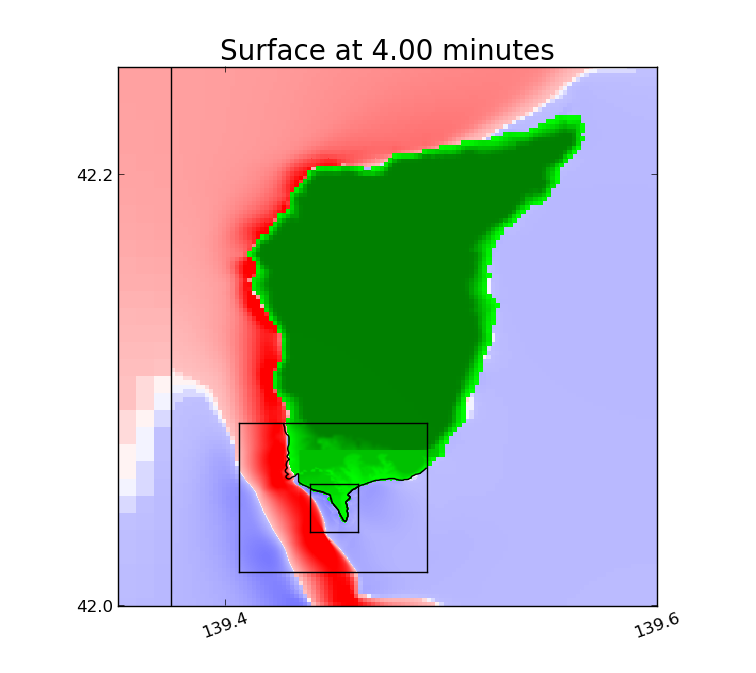
\includegraphics[width=2.0in]{bp9/ok_4min.png}\hfil
\hfil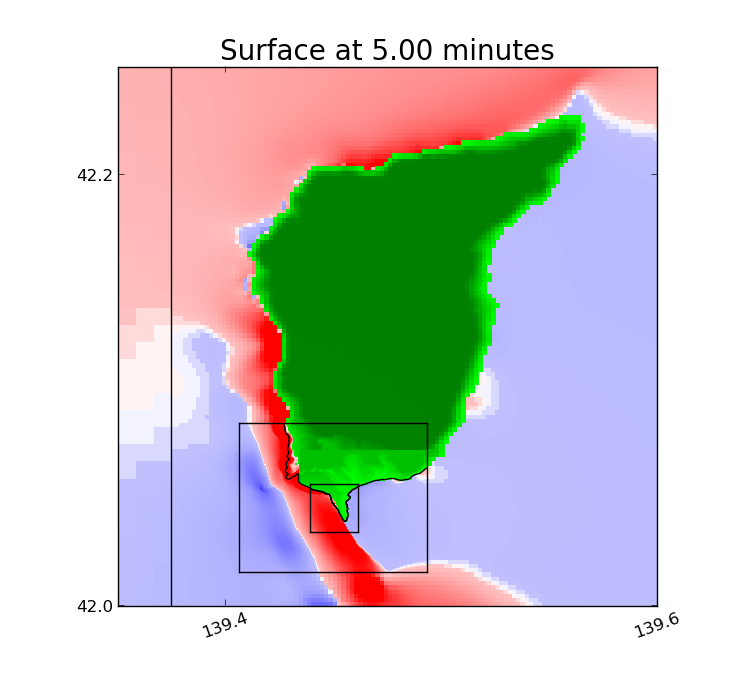
\includegraphics[width=2.0in]{bp9/ok_5min.png}\hfil
\vskip 10pt
\hfil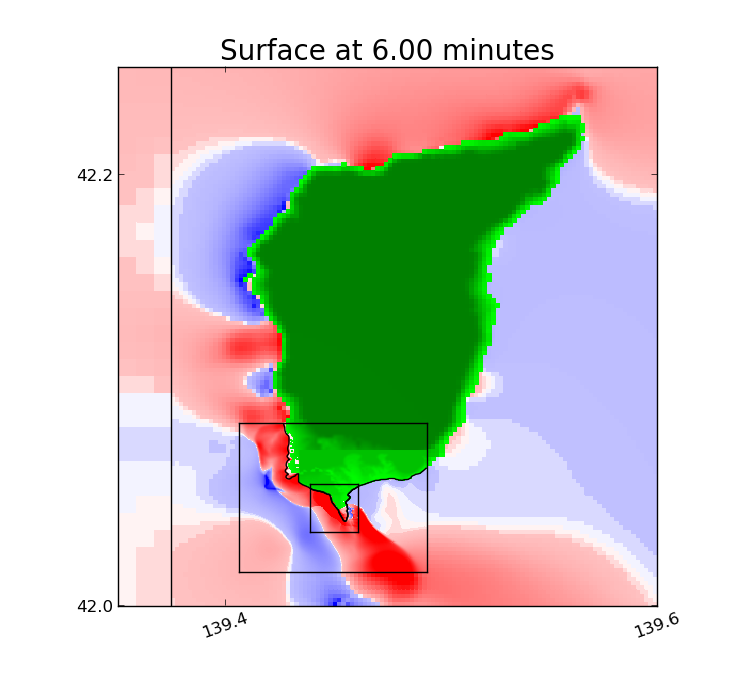
\includegraphics[width=2.0in]{bp9/ok_6min.png}\hfil
\hfil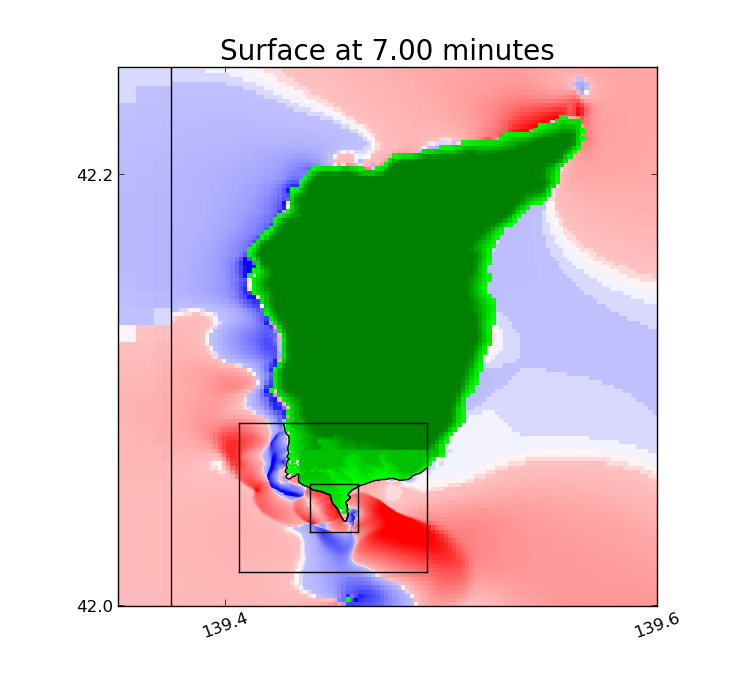
\includegraphics[width=2.0in]{bp9/ok_7min.png}\hfil
\hfil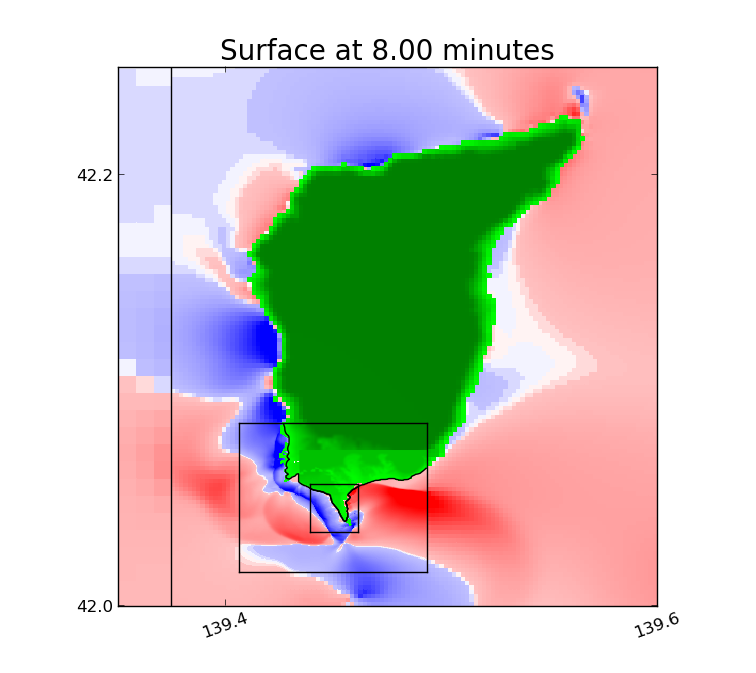
\includegraphics[width=2.0in]{bp9/ok_8min.png}\hfil
\vskip 10pt
\hfil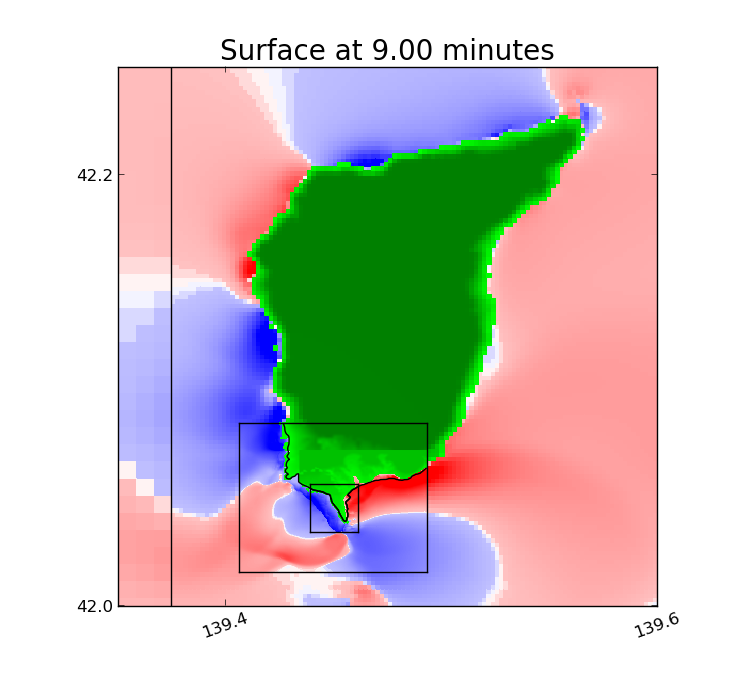
\includegraphics[width=2.0in]{bp9/ok_9min.png}\hfil
\hfil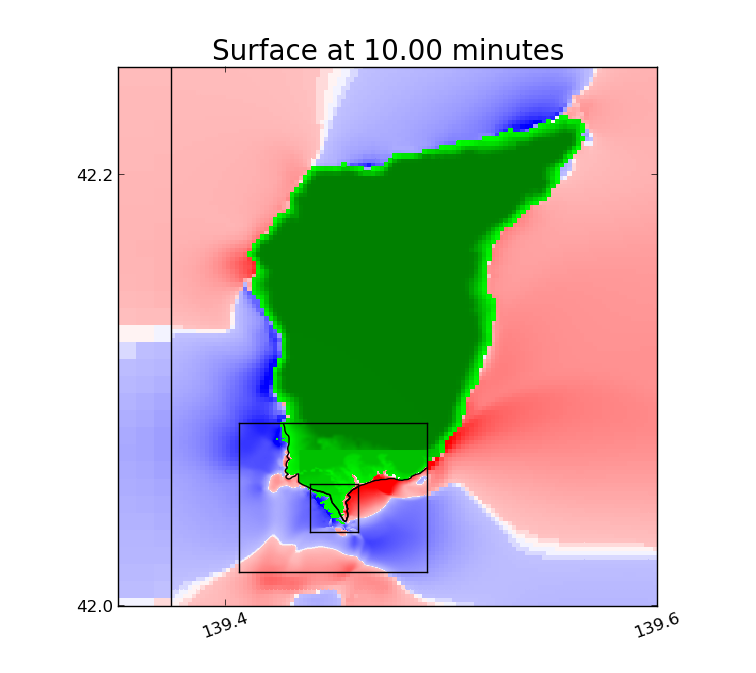
\includegraphics[width=2.0in]{bp9/ok_10min.png}\hfil
\hfil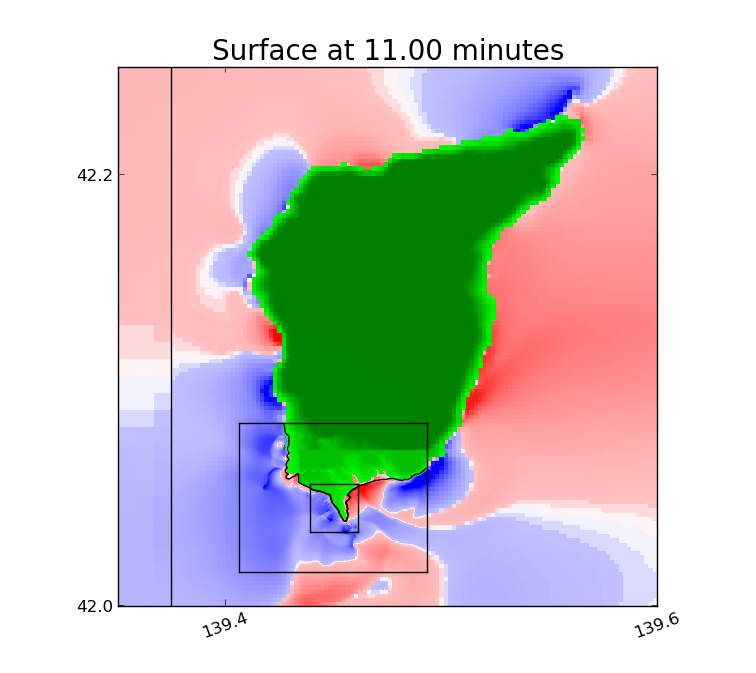
\includegraphics[width=2.0in]{bp9/ok_11min.png}\hfil
\caption{\label{bp9ok}
Zoom on Okushiri Island.
  }
\end{figure}

\begin{figure}[ht]
\hfil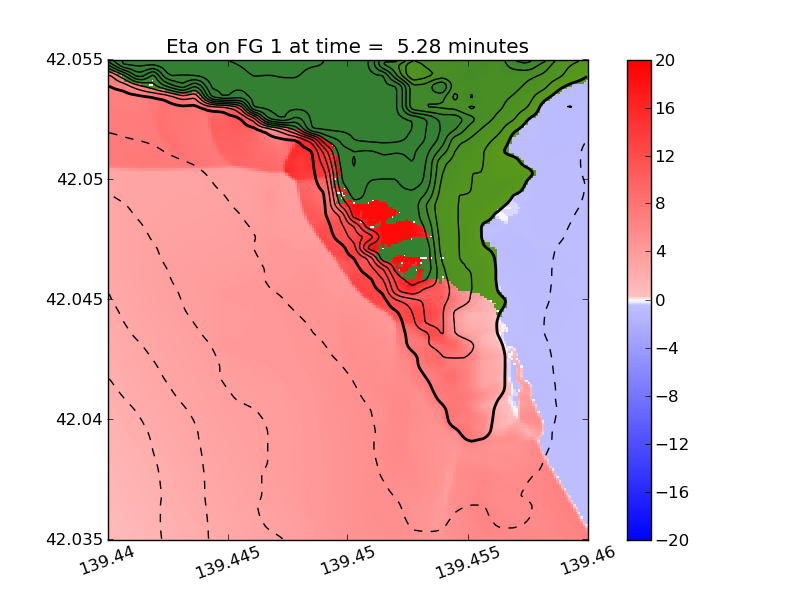
\includegraphics[width=2.8in]{bp9/aonae_5.png}\hfil
\hfil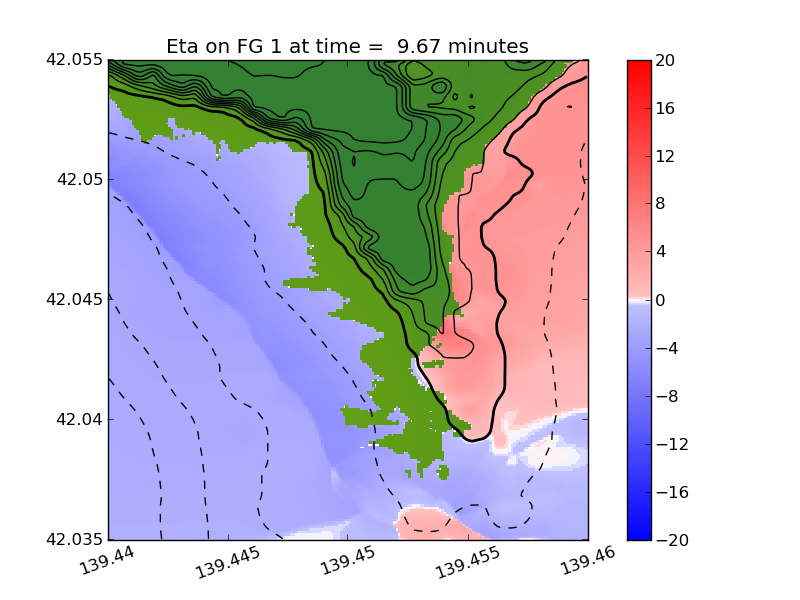
\includegraphics[width=2.8in]{bp9/aonae_14.png}\hfil
\caption{\label{bp9aonae}
Zoom on Aonae Peninsula showing the first wave arriving from the east and the second from the west.  Color map shows elevation of sea surface.  4-meter contours of bathymetry and topography are shown.
  }
\end{figure}

\begin{figure}[ht]
\hfil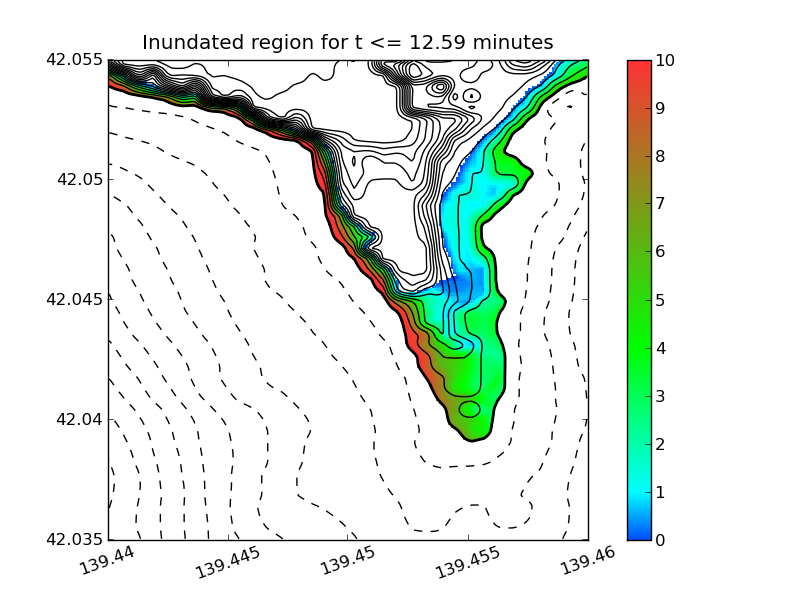
\includegraphics[width=5.0in]{bp9/in_aonae.png}\hfil
\caption{\label{bp9inaonae}
Inundation map of the Aonae Peninsula.  Color map shows maximum fluid depth over entire computation at each point. 4-meter contours of bathymetry and topography are shown. 
  }
\end{figure}

\begin{figure}[ht]
\hfil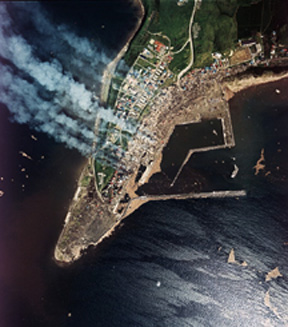
\includegraphics[width=2.8in]{bp9/AonaePhoto.jpg}\hfil
\hfil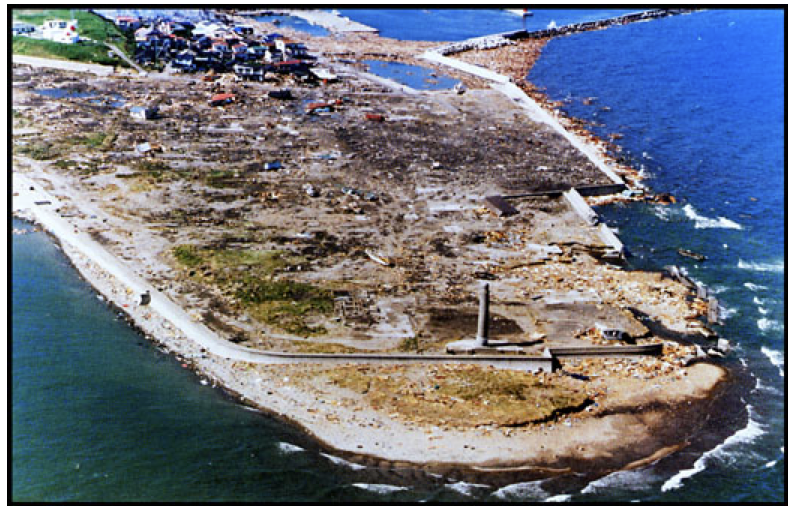
\includegraphics[width=2.8in]{bp9/AonaePhoto2.png}\hfil
\caption{\label{bp9photos}
Photographs of the Aonae Peninsula taken shortly after the event. \\
Left: From \protect\url{http://www.usc.edu/dept/tsunamis/hokkaido/aonae.html}. \\
Right: From \protect\url{http://nctr.pmel.noaa.gov/okushiri\_devastation.html}, credited to Y. Tsuji.
  }
\end{figure}

\begin{figure}[ht]
\hfil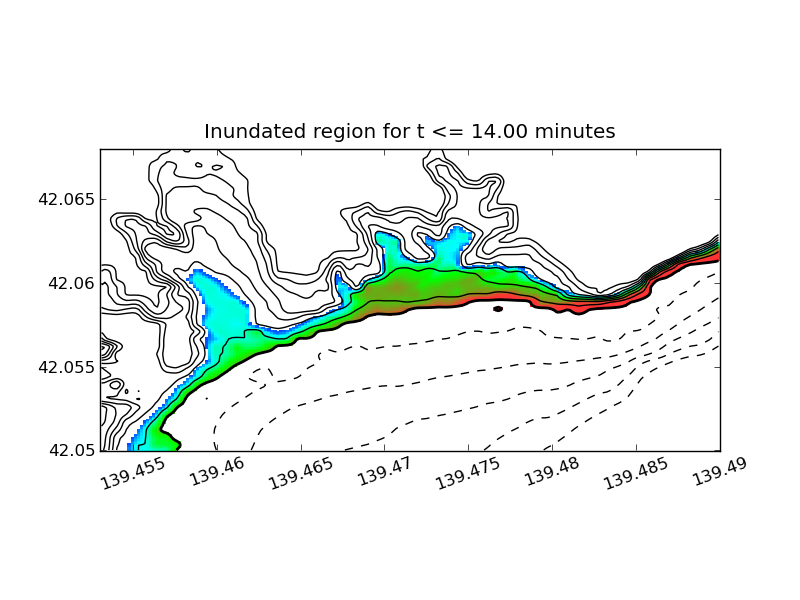
\includegraphics[width=5.0in]{bp9/hamatsumae.png}\hfil
\caption{\label{bp9hama}
Inundation map of the Hamatsumae neighborhood just east of the Aonae Peninsula.  Color map shows maximum fluid depth over entire computation at each point, with the same color scale as Figure \protect\ref{bp9inaonae}. 4-meter contours of bathymetry and topography are shown. 
  }
\end{figure}

\begin{figure}[ht]
\hfil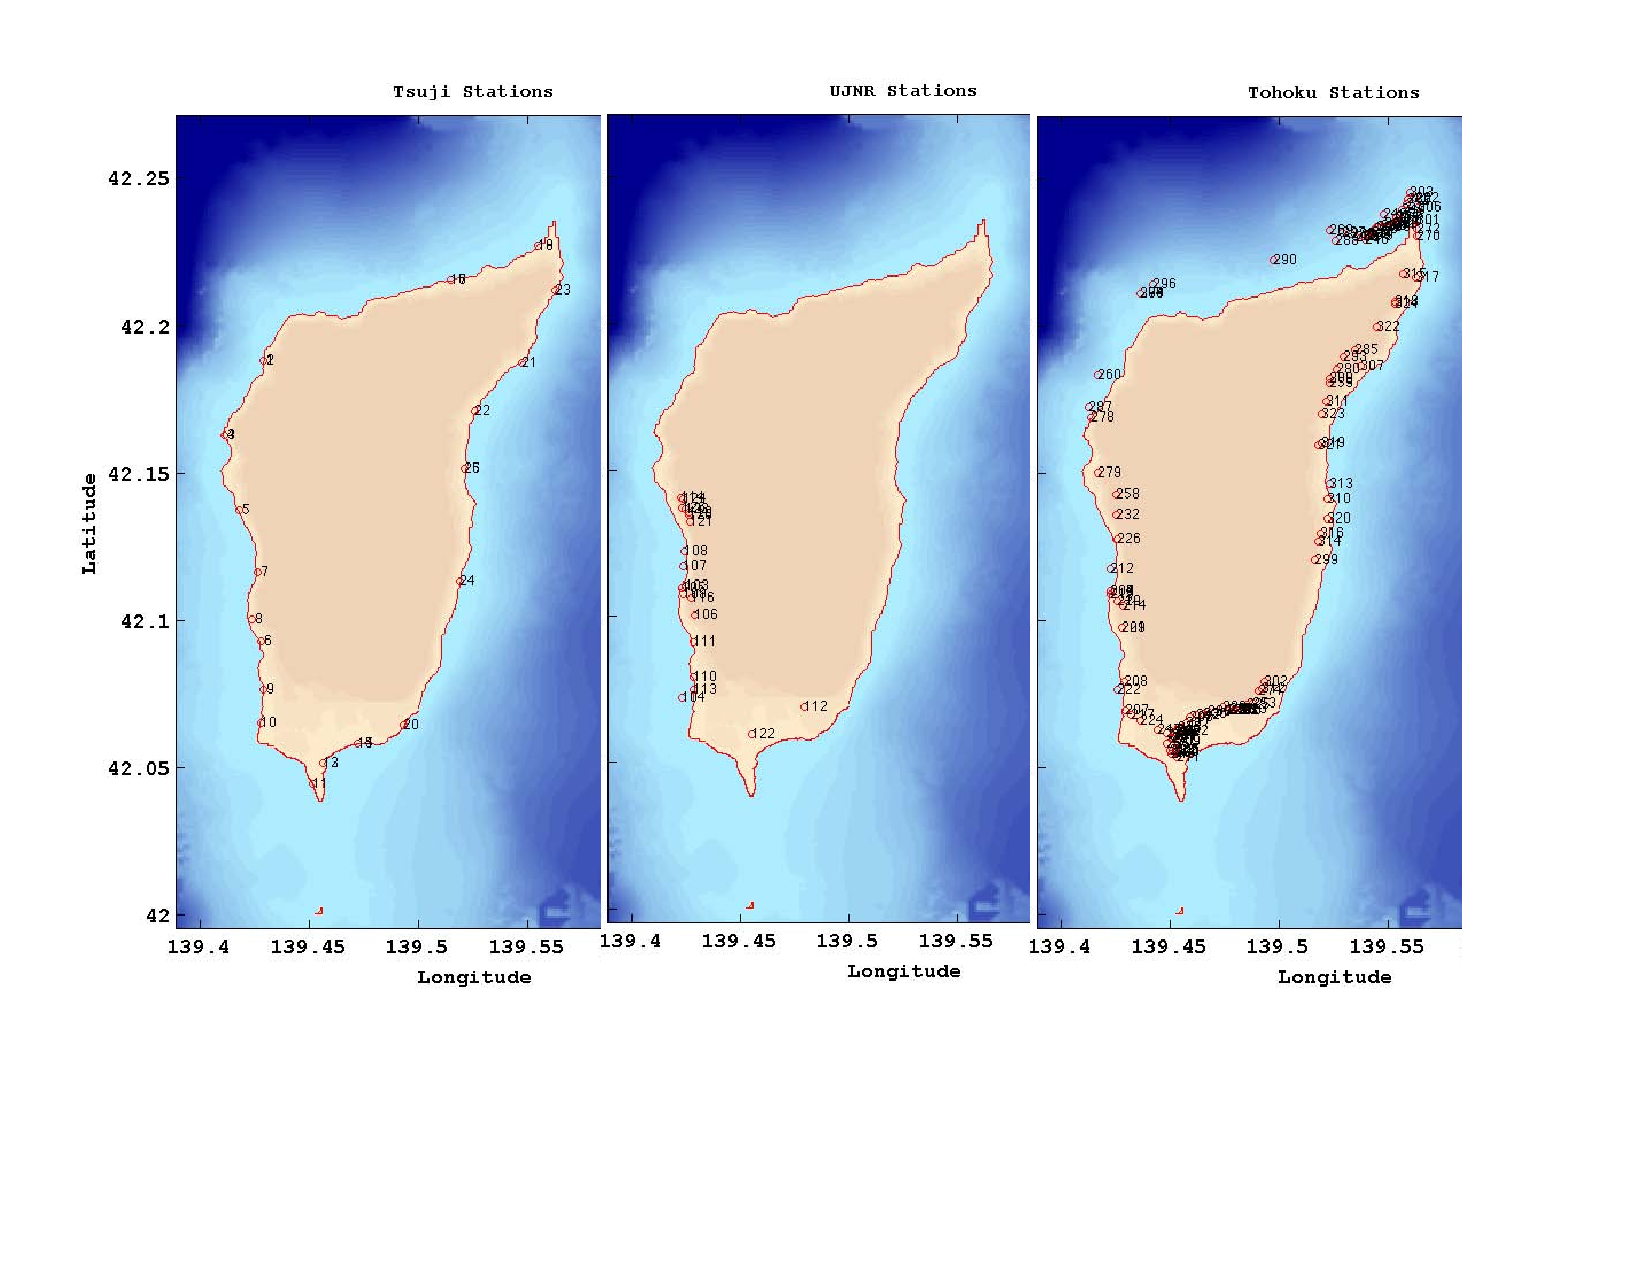
\includegraphics[width=5.0in]{bp9/TeamStations.pdf}\hfil
\vskip 10pt
\hfil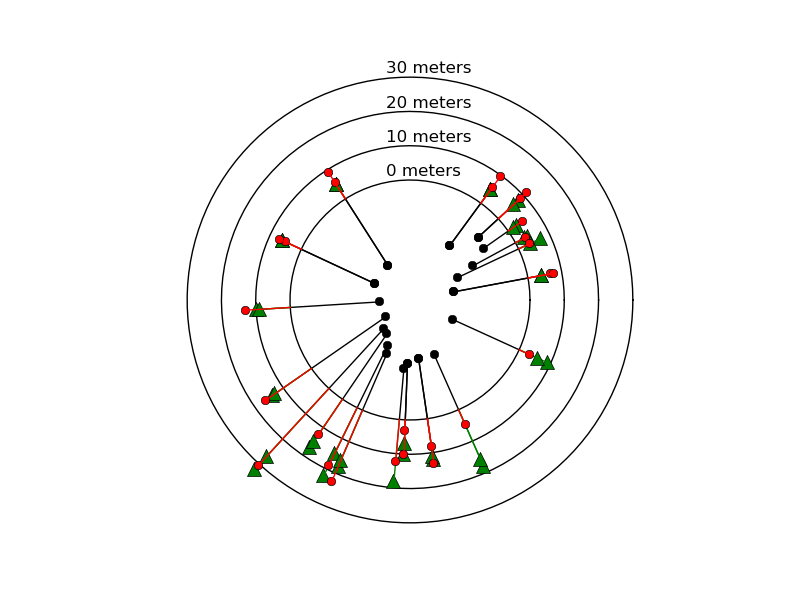
\includegraphics[width=5.0in]{bp9/runups.png}\hfil
\caption{\label{TeamStations}
Top: Locations of field observations by three independent field survey teams, relative to the computational bathy/topo grid system. Only the observations of Tsuji (left figure) were used in this study due to mis-registration of the other two data sets.\\
Bottom: Measured and computed runup at 21 points around Okushiri Island where measured by the Tsuji team.  Red circles are measurements, green diamonds are estimated from the computation.  Two red circles at the same point represent estimates of minimum and maximum inundation observed near the point.  Two green diamonds at the same point represent values estimated when the model was run with and without bottom friction (Manning coefficient 0.025).  The runup computed with bottom friction is the smaller value.
  }
\end{figure}


% \begin{figure}[ht]
% \hfil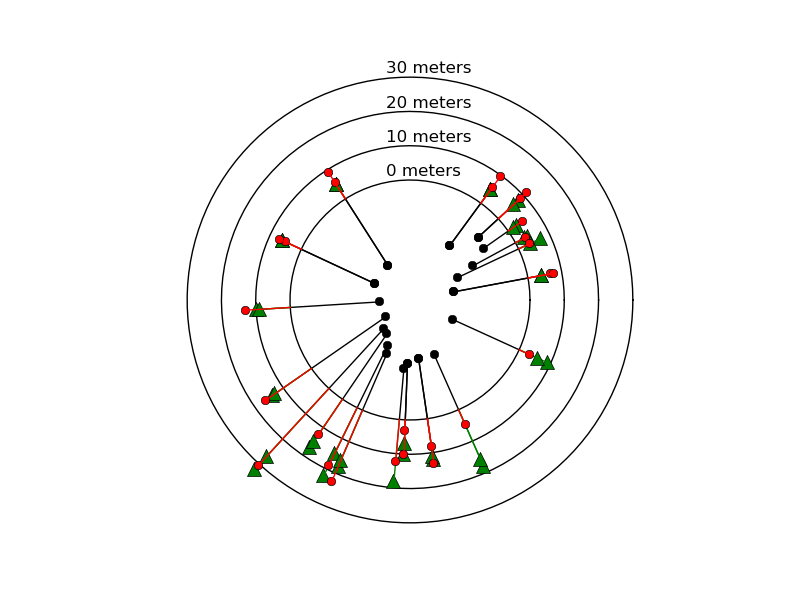
\includegraphics[width=5.0in]{bp9/runups.png}\hfil
% \caption{\label{bp9runups}
% Measured and computed runup at 21 points around Okushiri Island where measured by the Tsuji team.  Red circles are measurements, green diamonds are estimated from the computation.
%   }
% \end{figure}

\begin{figure}[ht]
\hfil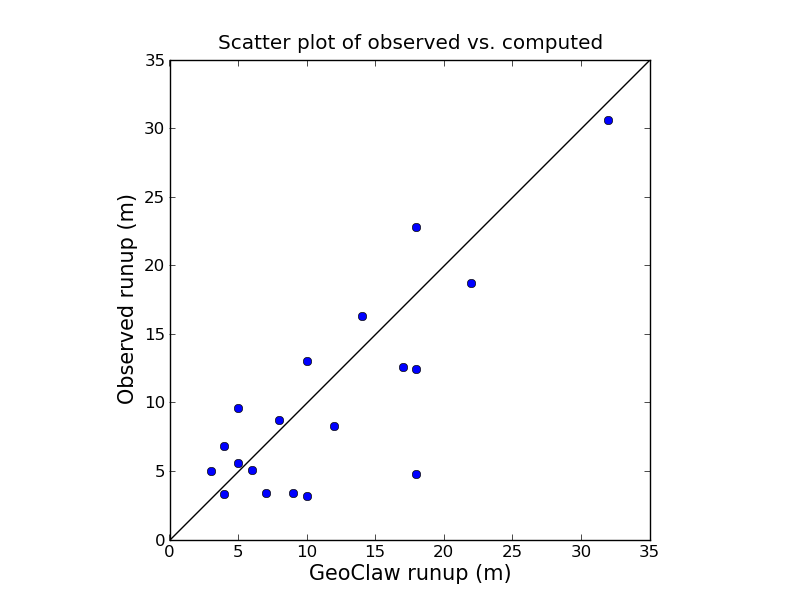
\includegraphics[width=2.8in]{bp9/scatter.png}\hfil
\hfil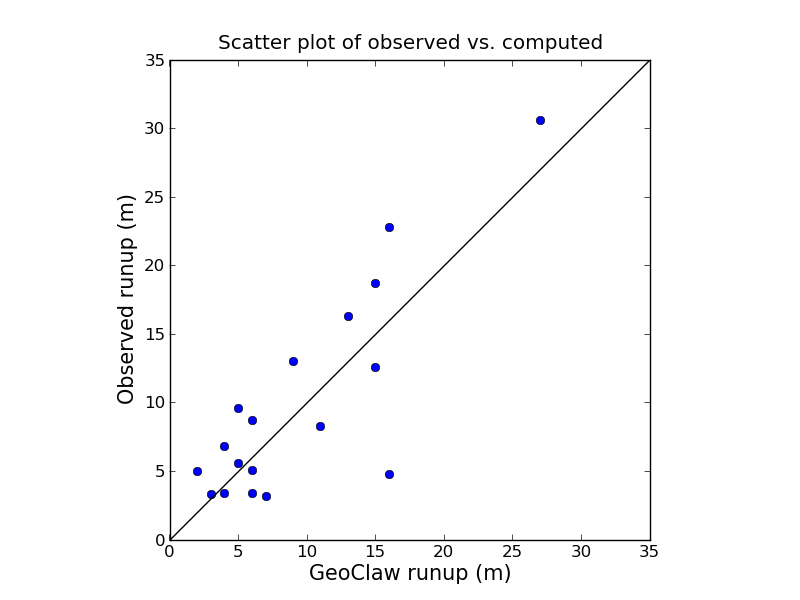
\includegraphics[width=2.8in]{bp9/scatter_friction.png}\hfil
\caption{\label{bp9scatter}
Scatter plot illustrating the correlation between measured and computed
values for the values shown in Figure \ref{TeamStations}.
Left: Without friction, Right: With Manning coefficient 0.025.
  }
\end{figure}

% \begin{figure}[ht]
% \hfil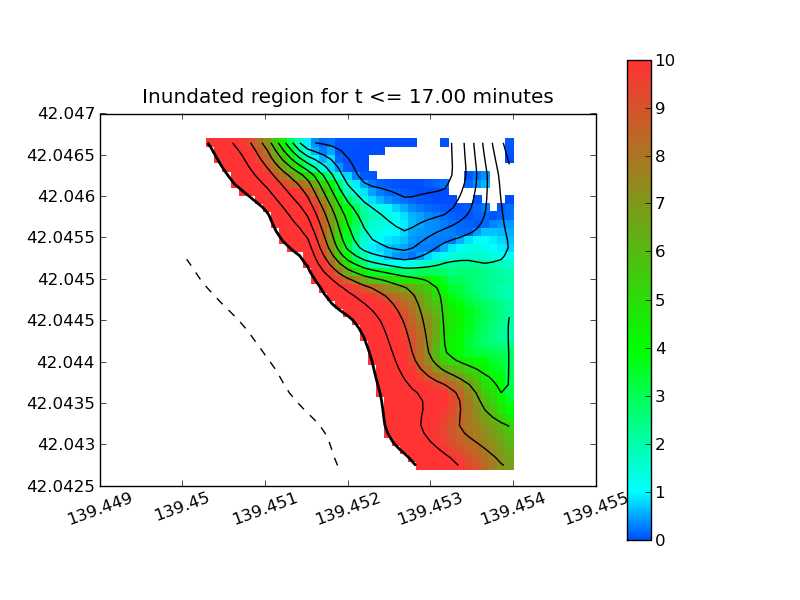
\includegraphics[width=2.8in]{bp9/in_11.png}\hfil
% \hfil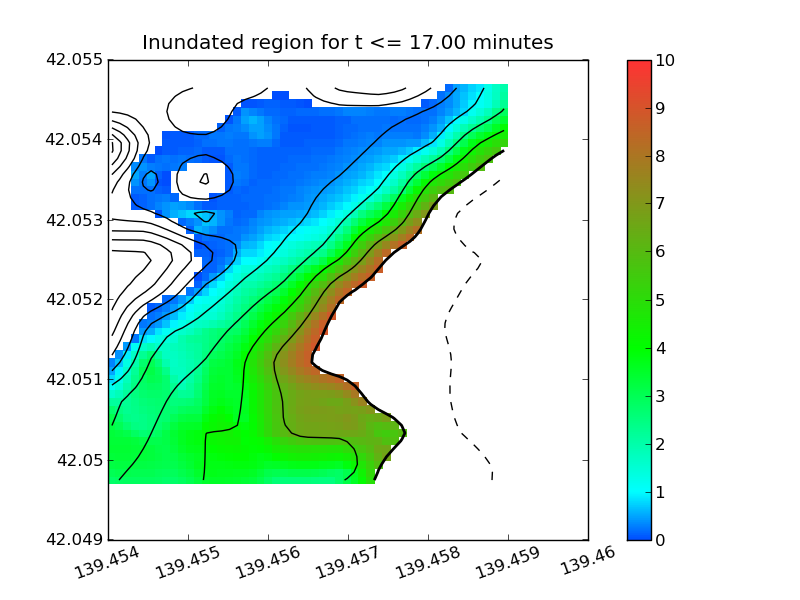
\includegraphics[width=2.8in]{bp9/in_12.png}\hfil
% 
% \caption{\label{bp9fg}
% Sample plots from which runup values are determined.
%   }
% \end{figure}

\begin{figure}[ht]
\hfil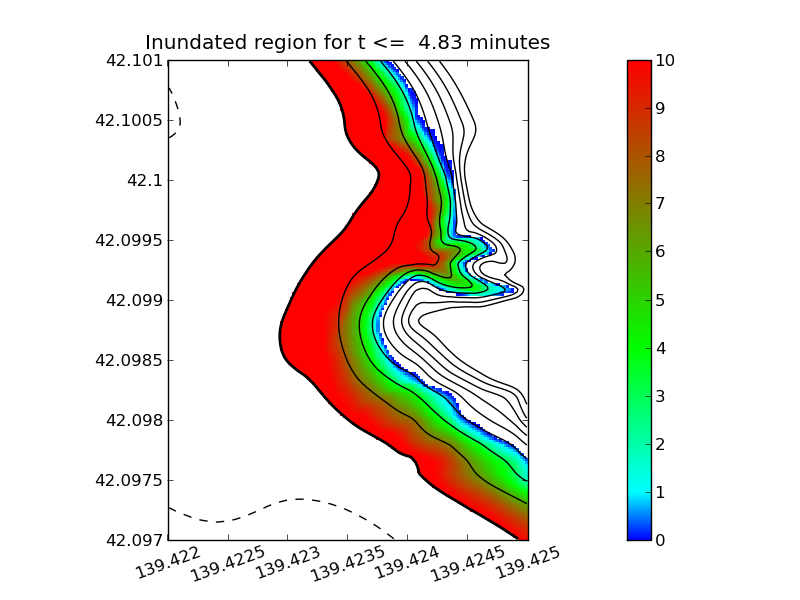
\includegraphics[width=4.0in]{bp9/in_monai_friction.png}\hfil
\caption{\label{bp9monai}
Inundation map of the valley north of Monai.  Color map shows maximum fluid depth over entire computation at each point. 4-meter contours of bathymetry and topography are shown. Compare to Figure \protect\ref{fig:bp7runup} showing the related wave tank simulation.
  }
\end{figure}

\begin{figure}[ht]
\hfil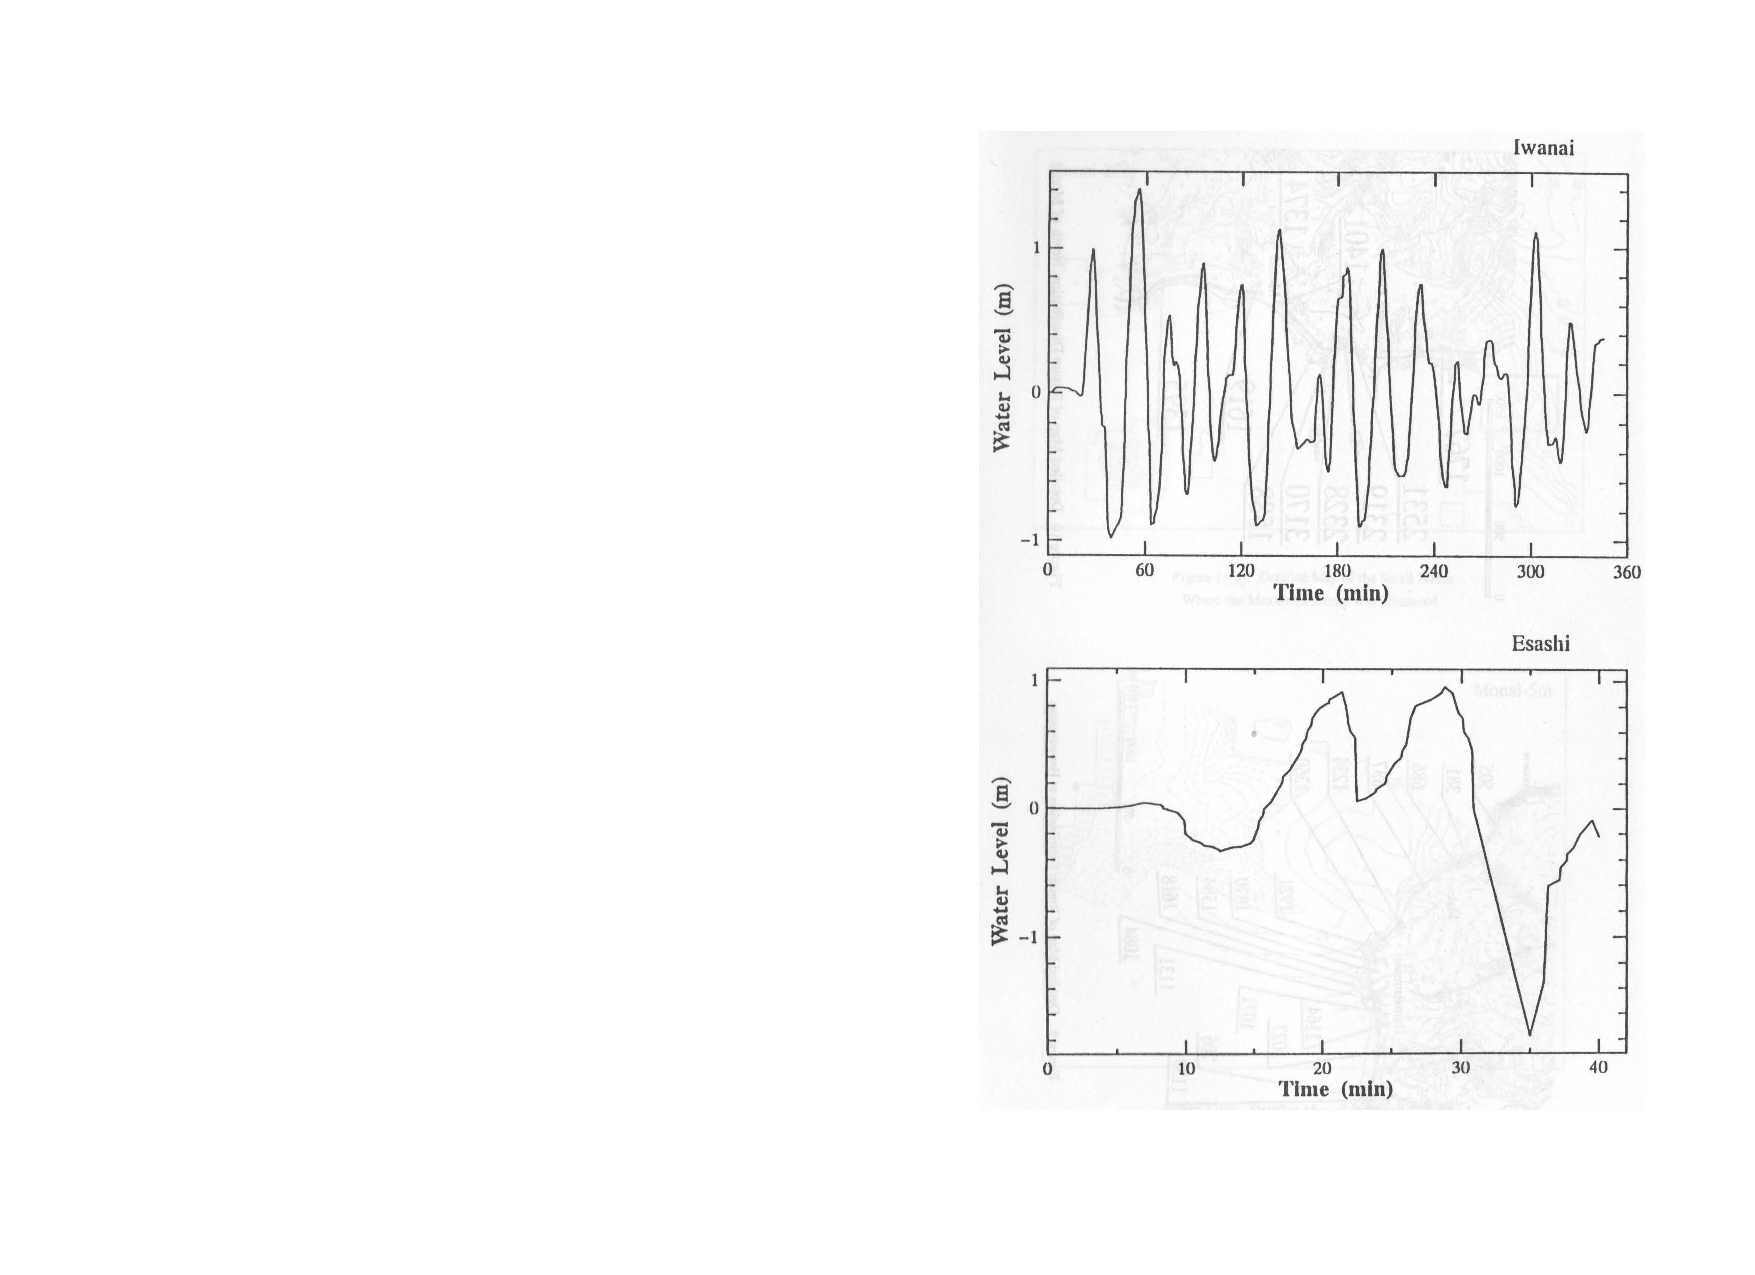
\includegraphics[width=5.0in]{bp9/TGs-Takahashi.pdf}\hfil
\caption{\label{TGs-Takahashi}
Analog tide gage records at Iwanai and Esashi.  (Faint background figures are a scanning artifact; the article is printed on paper that is not totally opaque.) 
  }
\end{figure}


\begin{figure}[ht]
\hfil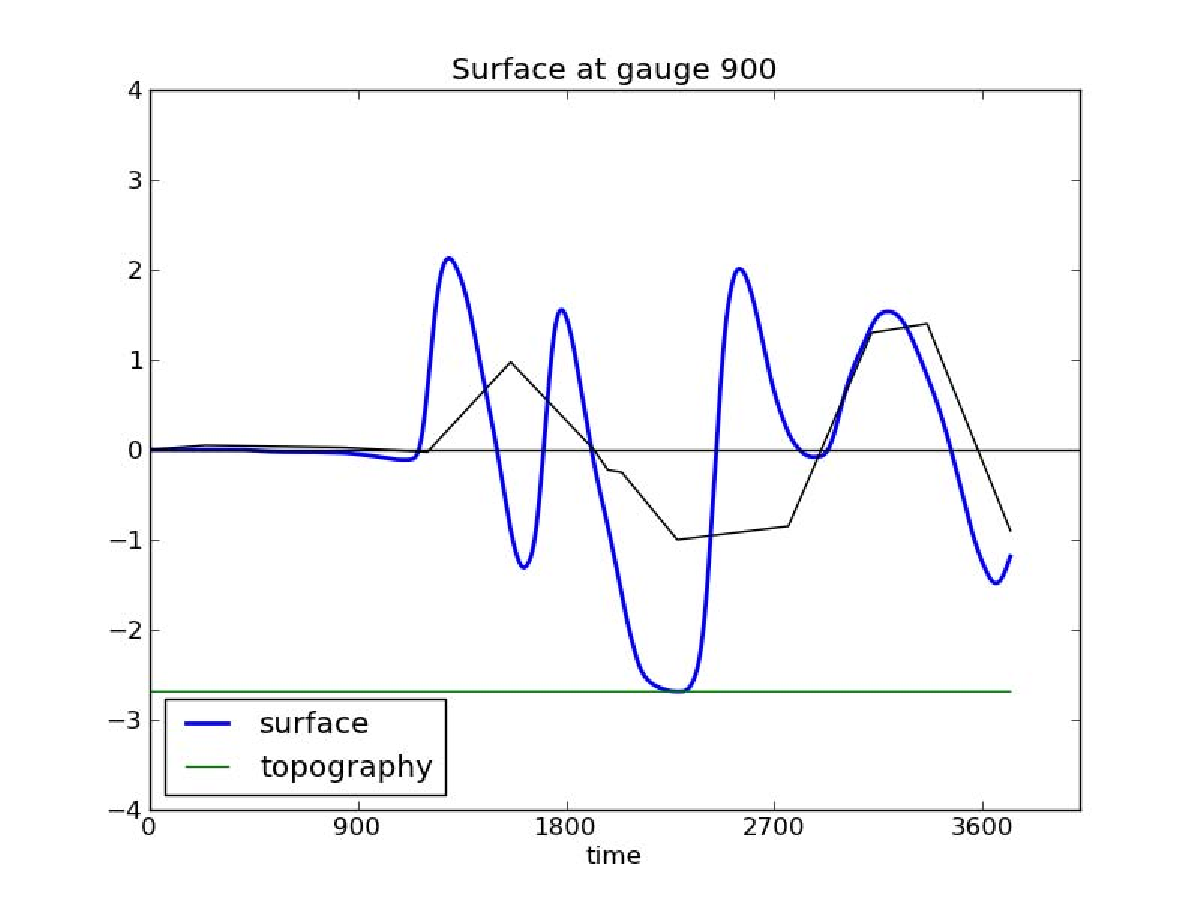
\includegraphics[width=5.0in]{bp9/Iwanai.pdf}\hfil
\caption{\label{Iwanai}
Iwanai digitized tide gage record (black line) and GeoClaw (blue line) time series. 
  }
\end{figure}

\begin{figure}[ht]
\hfil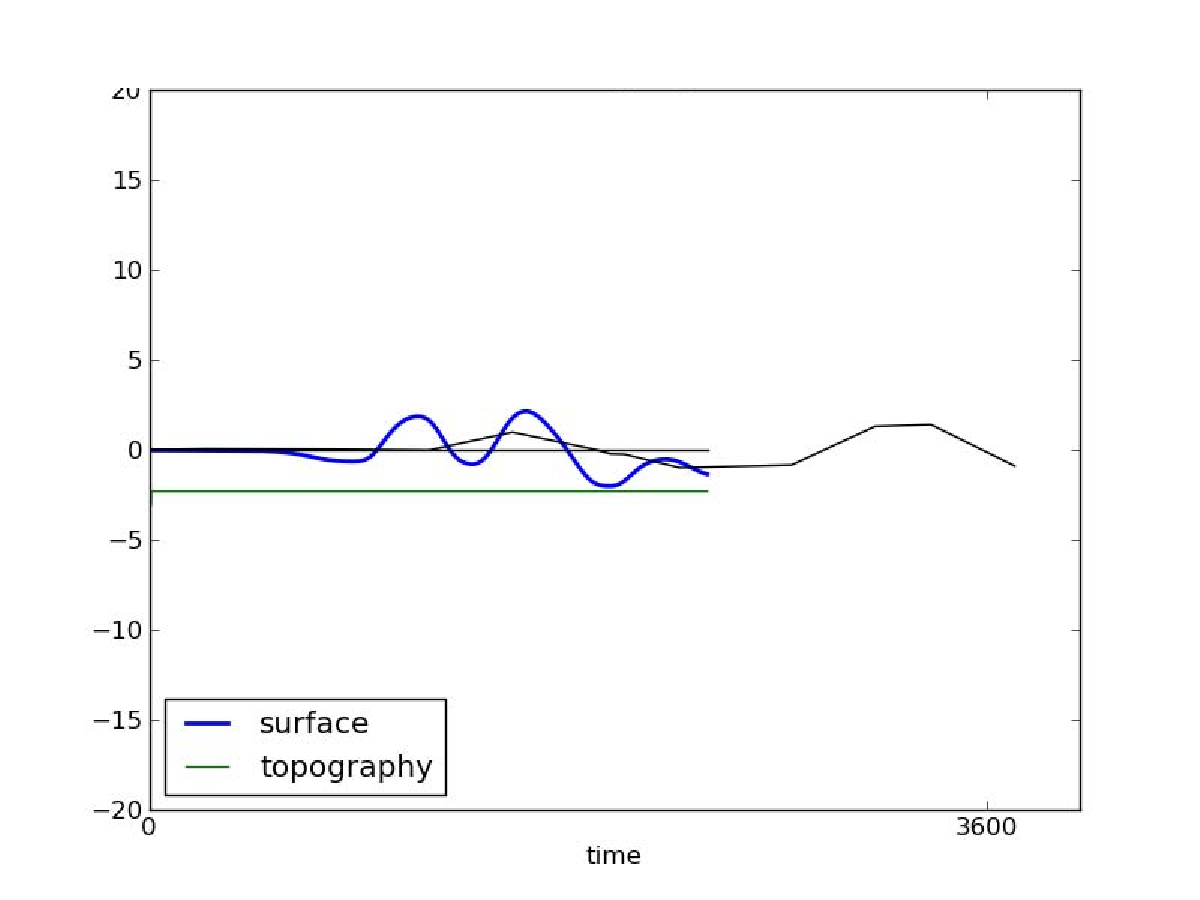
\includegraphics[width=5.0in]{bp9/Esashi.pdf}\hfil
\caption{\label{Esashi}
Esashi digitized tide gage record (black line) and GeoClaw (blue line) time series. 
  }
\end{figure}



\subsubsection{Lessons learned}
This BenchMark problem requires much more work to qualify as a credible test of tsunami inundation models.  We have little confidence in:
\begin{enumerate}
\item The quality of the bathy/topo computational grids.  A number of mismatches and discontinuities still exist in the system of grids.
\item The accuracy of the geospatial registration of observational data with model latitude and longitude positions.  Figure \ref{TeamStations} presents the observation locations of each of three field survey teams -- Professor Yoshinobu Tsuji, Tokyo University (Tsuji), the United States-Japan Cooperative Program on Natural Resources (UJNR) and the Tohoku University (Tohoku) teams.  The bathy/topo computational grids were adjusted to match the positions of the Tsuji observations, but it is clear that this created a systematic error in the registration of the grids with the Tohoku field observations and, in all likelihood, the UJNR field observations.  As another example, there appear to be discrepancies in the several field team reports of the latitude and longitude of the highest runup observed, i.e., the value of over 30 m in a `` ... small valley north of Monai ...".  Such positioning errors can be critical with respect to accurate comparisons of observed and computed runup.
\end{enumerate}

\subsubsection{Recommendations}
The Okushiri event tsunami runup and eyewitness reports remains one of the most valuable datasets for model comparisons in existence, but the quality of this dataset must be improved to qualify as a credible benchmark problem.  We recommend that an effort be supported to 
\begin{enumerate}
\item Develop a high quality bathy/topo grid system,
\item Resolve ambiguities and discrepancies currently found in the various team data reports, and improve the geospatial registration of observed and modeled values, and
\item Provide adequate documentation of the resulting benchmark problem dataset.
\end{enumerate}
